\section{Experiments}

The model has been tested in a series of benchmark environments, each with a different number of arms and reward distributions. The performance has been compared with the following algorithms: Random Baseline, Upper-Confidence Bound (UCB), Thompson Sampling, and Epsilon-Greedy.

% Description of the environments
\subsection{Game variants} \textbf{YEAH BUDDY WORK ON THIS A LIL MORE}

\noindent The game environments considered in this work are non-stationary K-Armed Bandits with Binomial rewards.
In particular, the agent is evaluated over a number $T_{\text{trials}}$ of \textit{trials}, each composed by an arbitrary number $T_{\text{rounds}}$ of \textit{rounds}; each \textit{trial} is characterized by a different reward distribution $\mathbf{p}\sim\mathcal{U}(0,1)^{K}$ (although in practice the bounds have been set to $(0.1, 0.9)$ such that the distributions are less trivial).
Our goal in this work is to investigate the performance of the agent in a non-stationary environment with Binomial reward distributions, meaning that its underlying distribution changes over time.
We choose this setting as it resembles an ecological scenario in which an animal has to forage in an environment with food (reward) is distributed over a set of fixed locations, but whose occurrence probability can change over time.
More specifically, we used four different variants:

\noindent \textbf{Zero-steps distribution shift} [\textsc{KAB-0}]: the reward distribution changes immediately at the end of a trial $i$ to a new one $i+1$ as $\mathbf{\mathbf{p}}_{i} \to \mathbf{\mathbf{p}}_{i+1}$.

\noindent \textbf{Epsilon-steps distribution shift} [\textsc{KAB-$\epsilon$}]:
the reward distribution $\mathbf{p}$ changes gradually over rounds, tracked as time $t$, such that its shape tends towards a target distribution $\mathbf{q}_{i}$ as
$\tau_{p}\dot{\mathbf{p}}_{t}=\mathbf{q}_{i}-\mathbf{p}_{t}$. Here, $\dot{\mathbf{p}}$ is the time derivative of the distribution and $\tau_{p}$ is its time constant.
Once distance is below a threshold $\epsilon$ as $\vert \mathbf{q}_{i} - \mathbf{p}_{t}\vert < \epsilon$, the target distribution is changed to a new one $\mathbf{q}_{i}\to\mathbf{q}_{i+1}$.

\noindent \textbf{Sinusoidal distribution shift} [\textsc{KAB-$\sin$}]: the reward distribution changes over rounds, with the probability of each arm following a sine wave with a specific frequency $f_{k}$, phase $\lambda_{k}$ and amplitude $1$. At any given time $t$, the distribution is $\mathbf{p}_{t}=\{\sin(2\pi f_{k}
t+\lambda_{k})\text{  for }k=1\ldots K\}$.

\noindent \textbf{Partial sinusoidal distribution shift} [\textsc{KAB-$\sin$P}]: identical to the sinusoidal distribution shift, but only a subset of the arms changes sinusoidally while the rest is kept at a constant value and the distribution is not normalized.


% Results: scores and brief discussion
\subsection{Environment variants and number of arms}

The model has been tested and compared with the other algorithms: Thompson Sampling, Epsilon-Greedy, and UCB, in the four different variants of the K-armed bandit problem.
In figure \ref{fig:perf_plot}, it is reported their results over a different number of arms, ranging from 5 to 1000.
Overall, our model displayed a remarkable performance over all environments and arm numbers, suffering only when the latter reached 1000.

\begin{figure}[H]
    \centering
    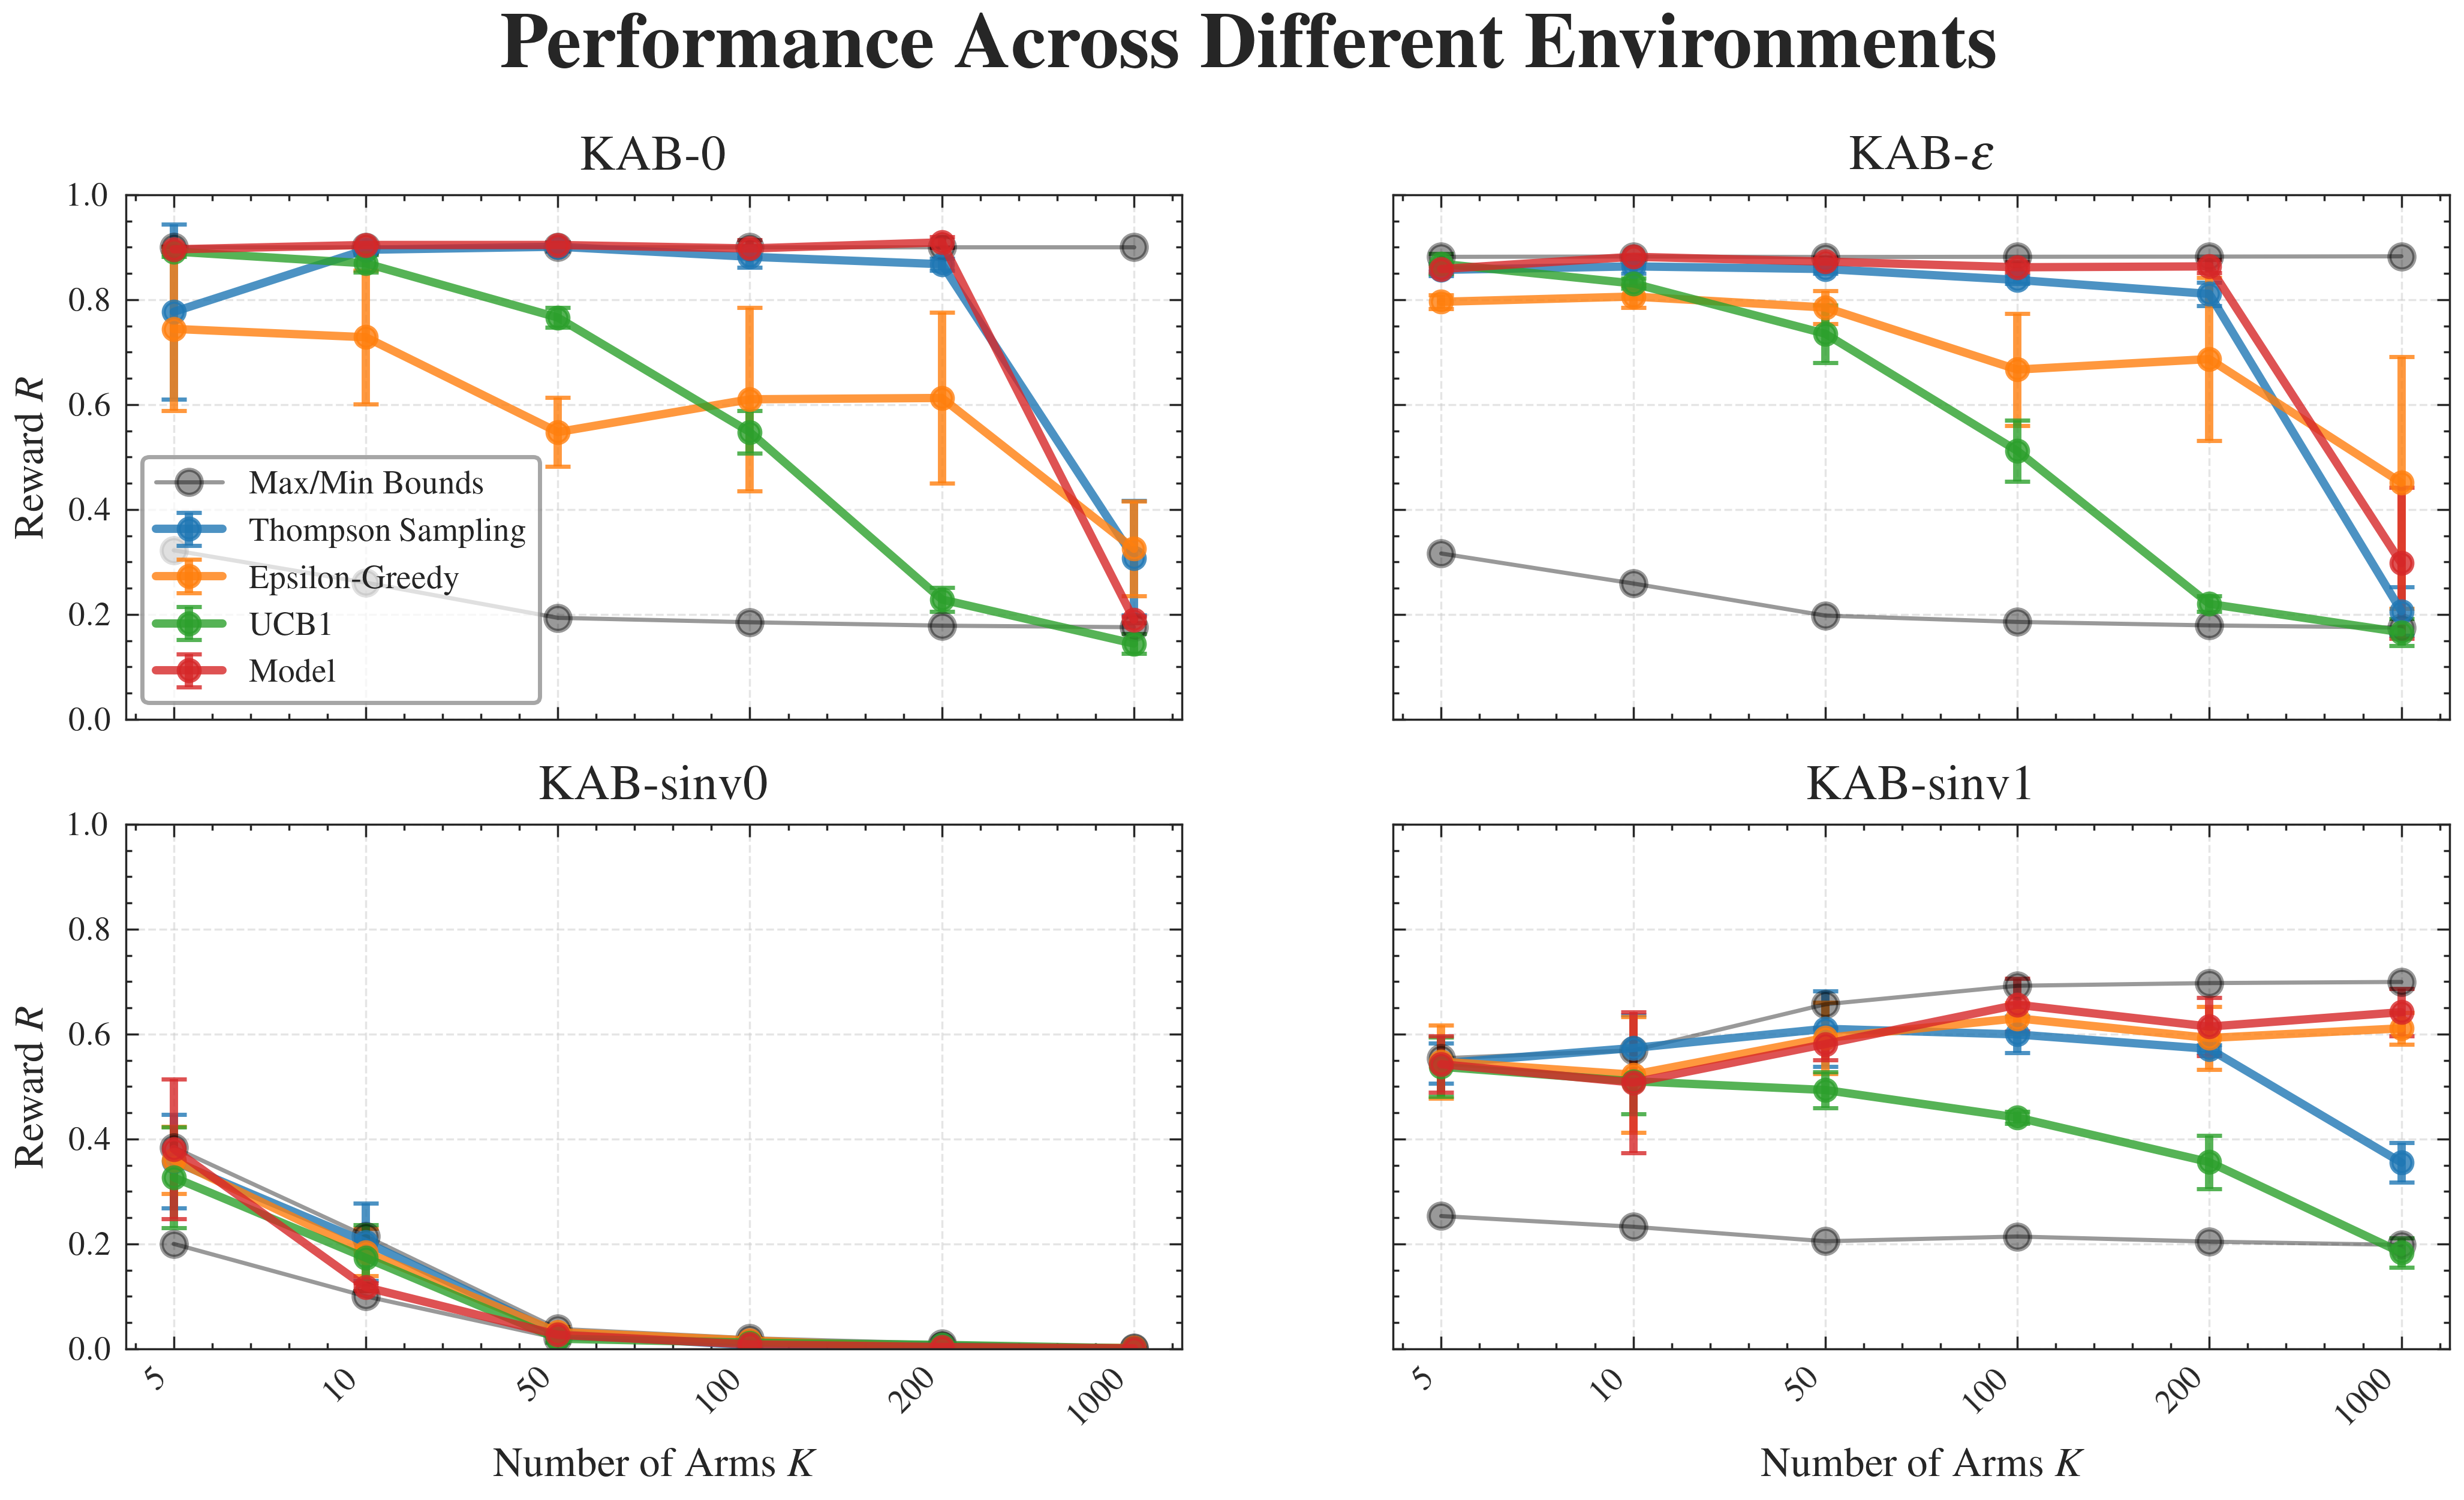
\includegraphics[width=1.\textwidth]{figures/performance_plot.png}
    \caption{\textsc{Performance comparison for different values of $K$ and game variants} - \textit{The models are evaluated on the four variants of the bandit problem, and their performance is measured as the average reward obtained over 2 trials of 2000 rounds each.}}
    \label{fig:perf_plot}
\end{figure}


% How the models work and compare
\subsection{Decision-making dynamics}

% entropy over rounds
\subsubsection{Entropy analysis}\label{sec:entropy}
\noindent For a better understanding of the qualitative differences between the models, we analyzed the progress over the rounds by tracking the selected arms, within the simplest case of zero-steps distribution shift.
Additionally, in order to quantify the variability of the decision policy at a given time and highlight the particularity of each decision-making behaviour, we calculated the entropy of the probability distribution $p$ of chosen arms, calculated over a window of 20 rounds, as $H=-\sum^{K}_{i} p_{i}\log(p_{i})$.
The unit of entropy is in nats, and it ranges from $0$ (no uncertainty) to $\log_{e}(K)$ (maximum uncertainty).
In figure \ref{fig:entropy_fig1}, it is plotted for each model the raster plot of selected arms together with its level of entropy. The reward probability distribution over the arms has $H=2.02$.

As expected, the shape of the entropy curve expresses the inherent strategy adopted by each model.
In particular, the UCB algorithm showed the highest variability, marked by a persistent exploratory behaviour throughout the trials despited converging to reward options. Thompson Sampling was able to reach most solutions, although with difficulty in adapting to new reward distributions
leading to high entropy levels.
$\epsilon-$Greedy also showed a good performance quite reliably, with the greedy strategy assuring low entropy for most of the rounds.
Similar behaviour was observed for our model, which was able to reach the optimal policy and maintain it over time, with entropy peaking mostly at the beggining of the trials and being, on average, the lowest among all models.
Indeed, the dynamics of our model make it particularly suited for the task of non-stationary K-armed bandits, as it is able to quickly adapt to new reward distributions and firmly maintain a greedy policy.

\begin{figure}[H]
    \centering
    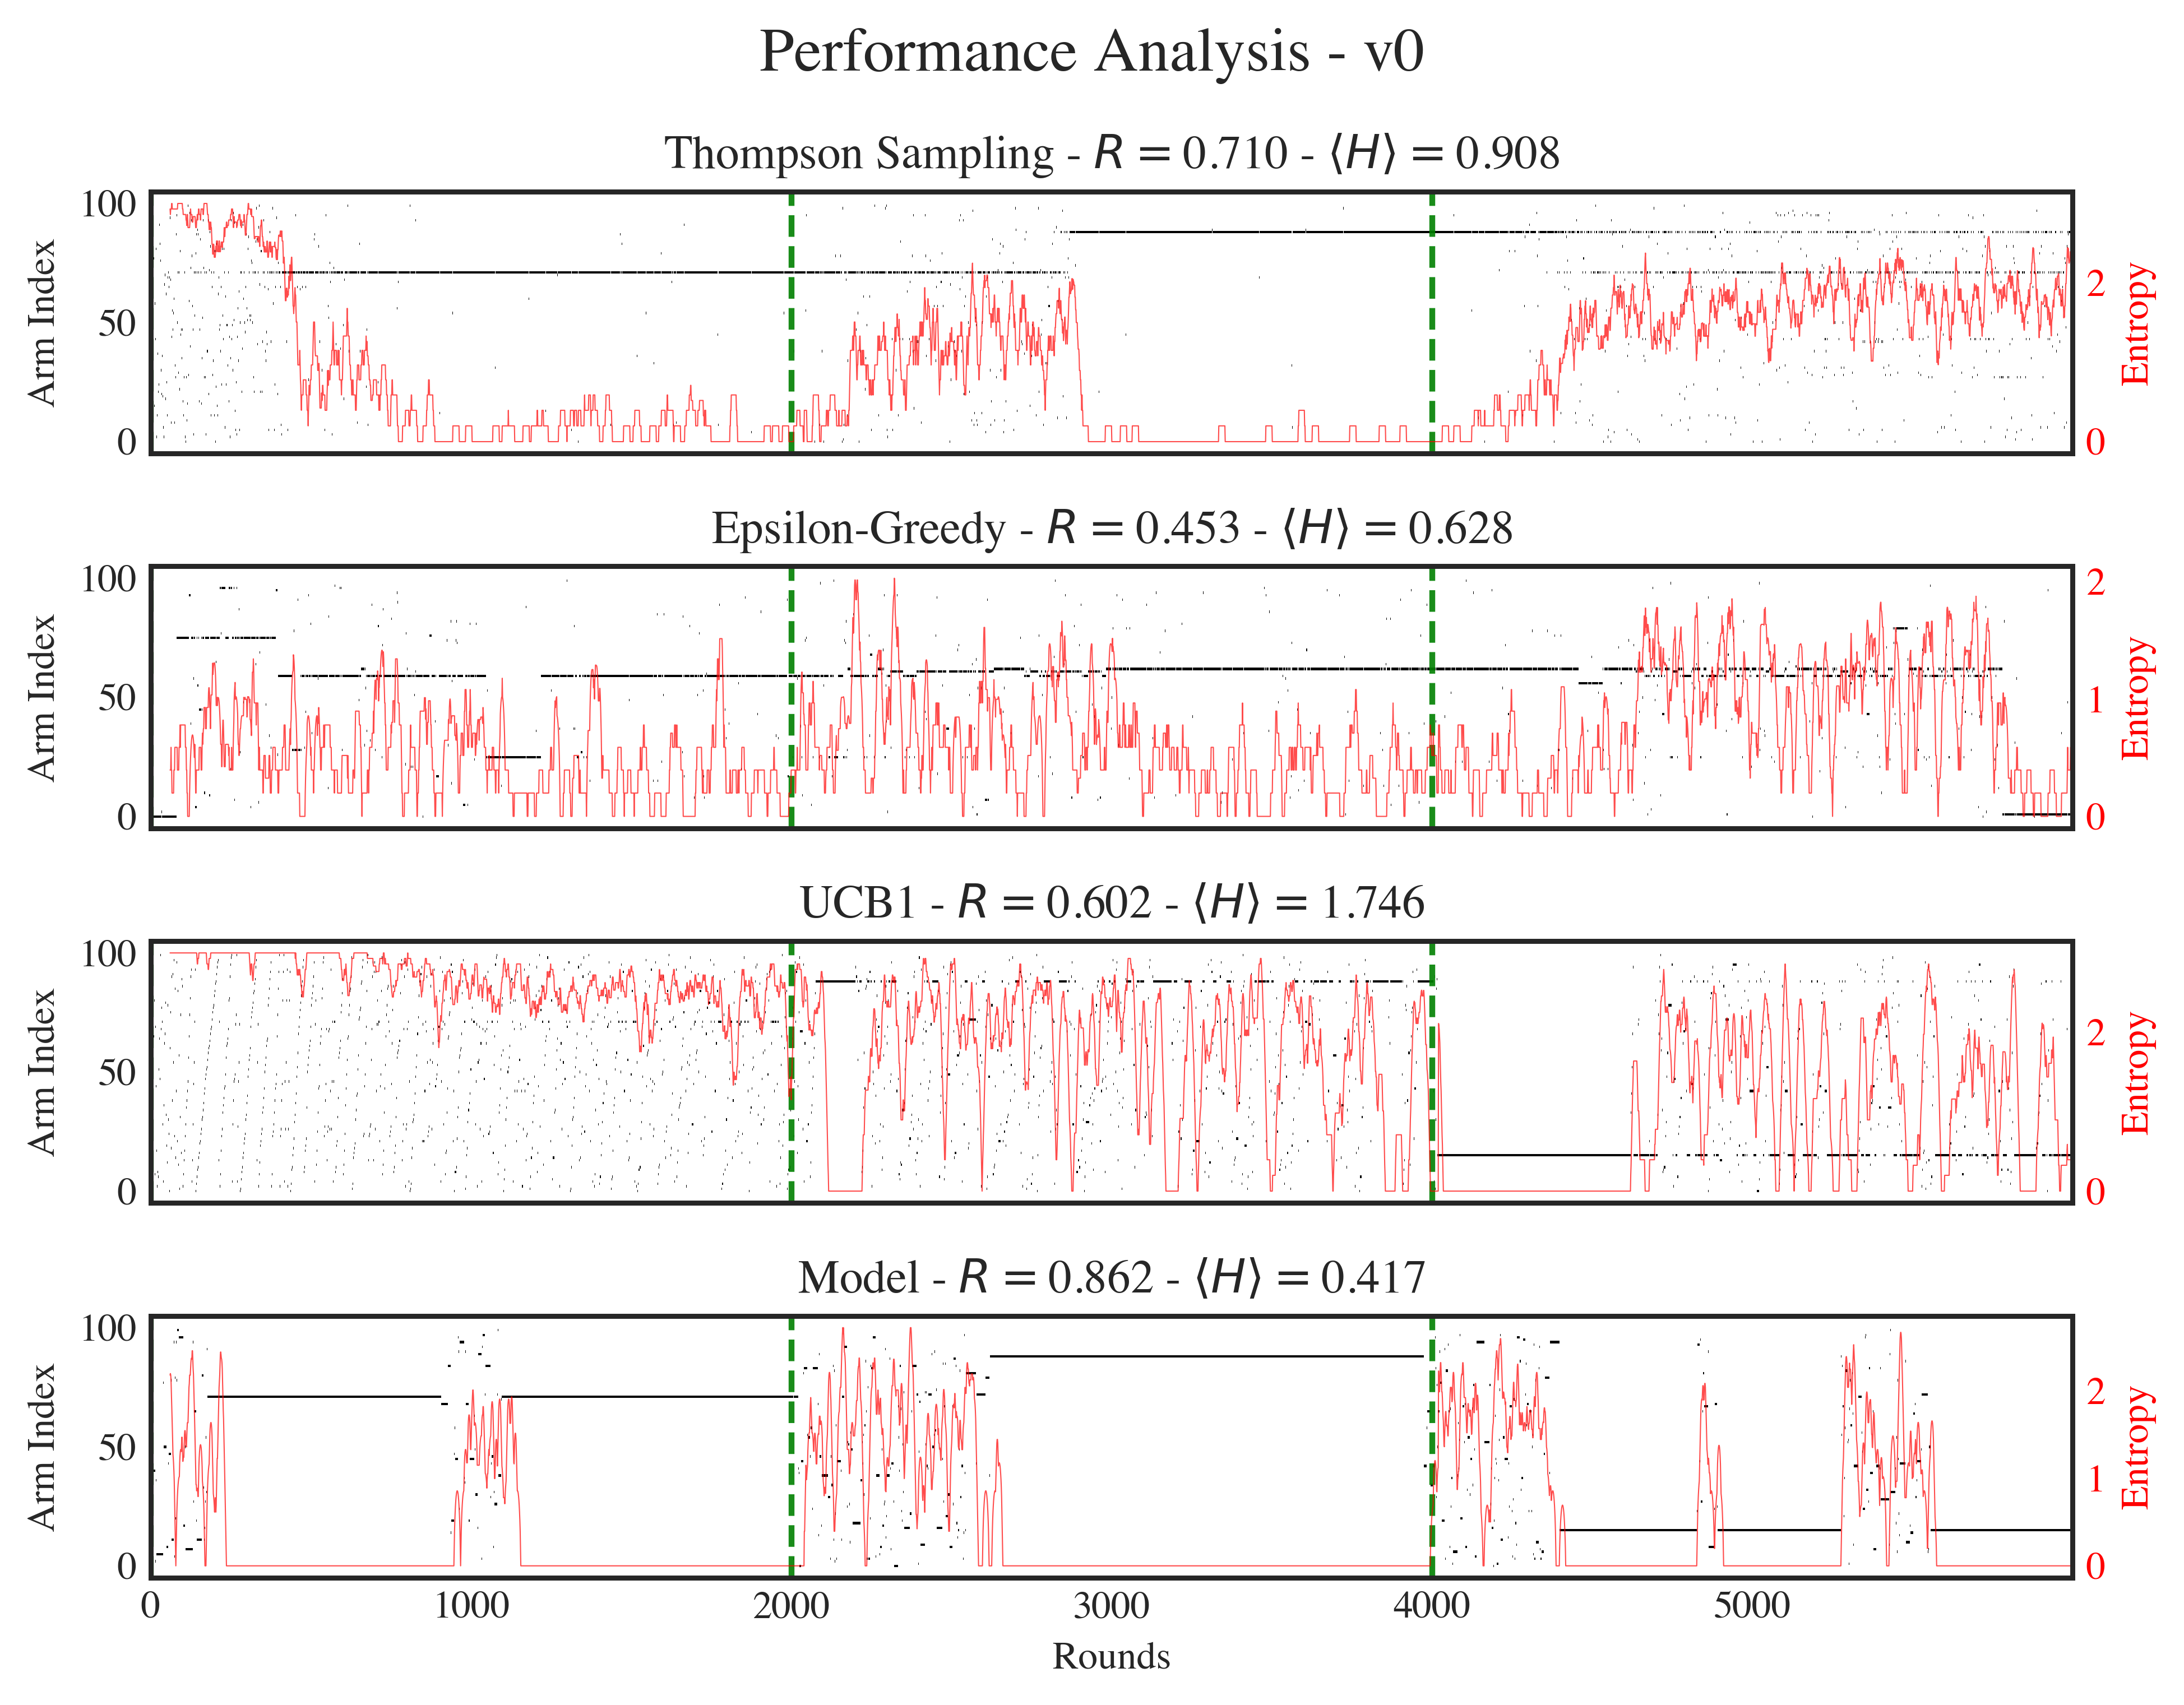
\includegraphics[width=1.0\textwidth]{figures/performance_analysis_KABv0.png}
    \caption{\textsc{Decision-making dynamics for different models} \textit{Each plot display the results from one model. The raster plots (black dots) show the arms selected at each round.
The red lines represent the entropy level, calculated from the distribution of selections over the preceeding 20 rounds, smoothed with a 30-steps moving average. In the plot titles, the total reward and average entropy over all trials are also reported.}}
    \label{fig:entropy_fig1}
\end{figure}


% weight update over rounds
\subsubsection{Weight update dynamics}
\noindent Next, we analyzed the weight update dynamics of the model over the rounds.
In figure \ref{fig:rew_update}, we plotted the evolution of the weights for each arm over time, averaged over 20 simulations and smoothed over 30 rounds.
The results show that the model is able to quickly adapt to new reward distributions. It is also able to maintain the optimal policy over time, with the weights remaining approximately stable.
The update quantity $\Delta W_{k}^{UV}$ changes sign according to the collected reward, with its magnitude being higher at the beginning of the trials.
Initially, the sign is mostly positive (potentiation) since the weights start at zero, and after some uncertainty a consistently preferred arm emerges.
However, when the reward distribution switches a regular series of sub-optimal choices is made, leading to zero reward.
This causes an accumulation of weight updates with negative sign (depression), eventually bringing the value of the preferred arm to drop. In the meantime, other options are probed until another sequence of choices converges to another arm, promoted by a trail of positive weight updates.

This behaviour is consistent with the low entropy levels observed in the previous analysis.


\begin{figure}[H]
    \centering
    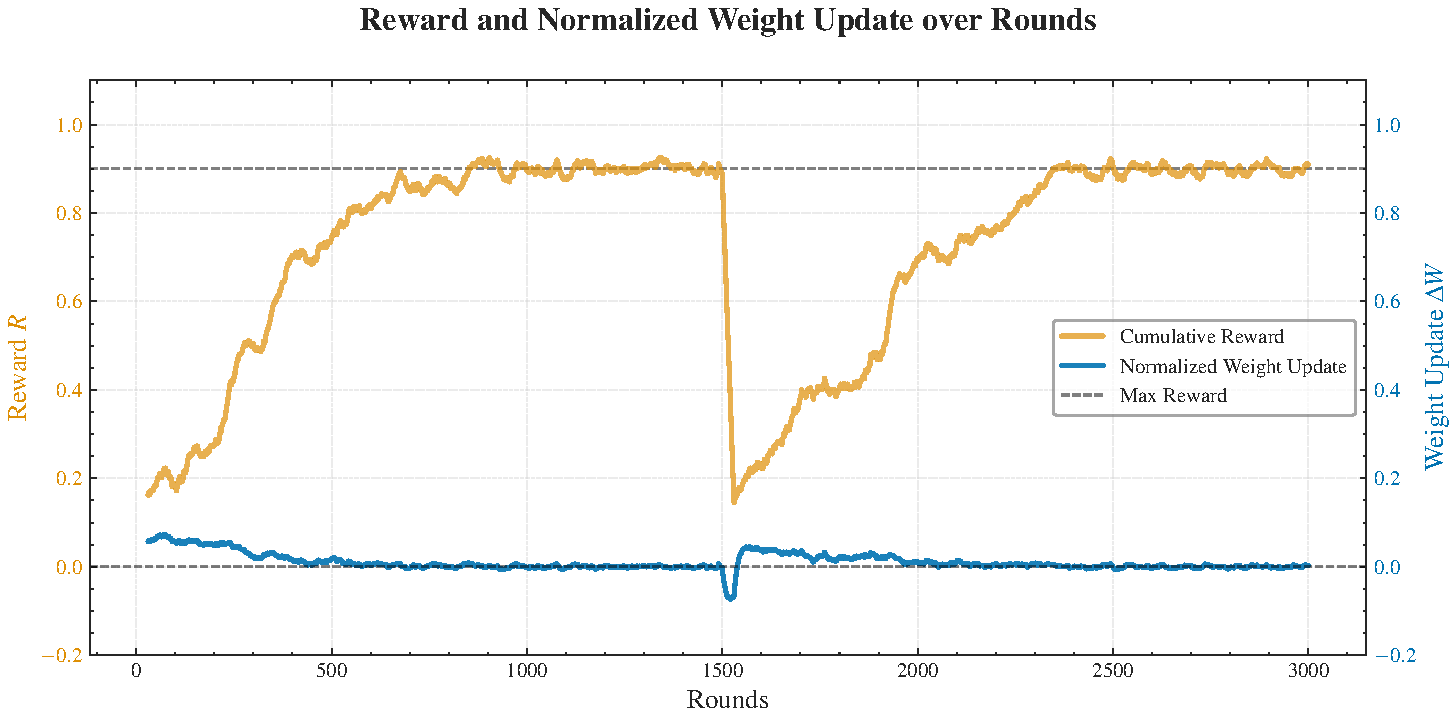
\includegraphics[width=1.0\textwidth]{figures/reward_update_plot.pdf}
    \caption{\textsc{Weight update developement for the model} \textit{The plot displays the weight update quantity $\Delta W_{k}^{UV}$ for each round (blue line), smoothed as a 20-steps moving average.
    It is also reported the average reward in a window of 30 rounds (golden line). The results have been obtained averaging over 20 iterations.}}
    \label{fig:rew_update}
\end{figure}


% how robust and structure is the model
\subsubsection{Robustness}

% robustness
\noindent Then, we sought to investigate the robustness of the model.
This was accomplished by evaluating the performances in a stationary setting with $K=50$ and increasing levels of entropy in the reward distribution, averaged over 128 simulations and again measured in nats.
For more details about the distribution see the appendix \ref{sec:appendix_entropy}.
In the top row of figure \ref{fig:entropy_distr}, it is plotted the average reward obtained by each model against the reward distribution entropy in two trials.
The results report how all models are capable of robust performance even in the presence of high uncertainty.
In the second trial however, there is a ubiquitous and clear decline in rounds of elevented entropy. This can be explained by the greated challenge of changing arms when numerous options appear similarly good.
In general, our model shows to perform as good as UCB, and better than Epsilon-Greedy and Thompson Sampling.
Further, the latter seemed to suffer the most, probably due to its conservative approach and difficulty of disengaging from an previously rewarding arm, as underlined also in figure \ref{fig:entropy_fig1}.
In the same figure, the regret (dashed lines) tells the same story, and remarks the robust performance over uncertainty.

Another perspective to this analysis is given by the plots in the bottom row, which show the average entropy of the selections.
Overall, there is the not suprising trend of increasing selection entropy with the entropy of the reward distribution. However, striking is the exception of Epsilon-Greedy, which maintain a constant level throughout.
On the one hand, UCB shows a marked and gradual increase, while Thompson Sampling follows with some delay.
On the other hand, our model display a more abrupt change, at around 2.43 nats, going from a state of very low to very high entropy.


\begin{figure}[H]
    \centering
    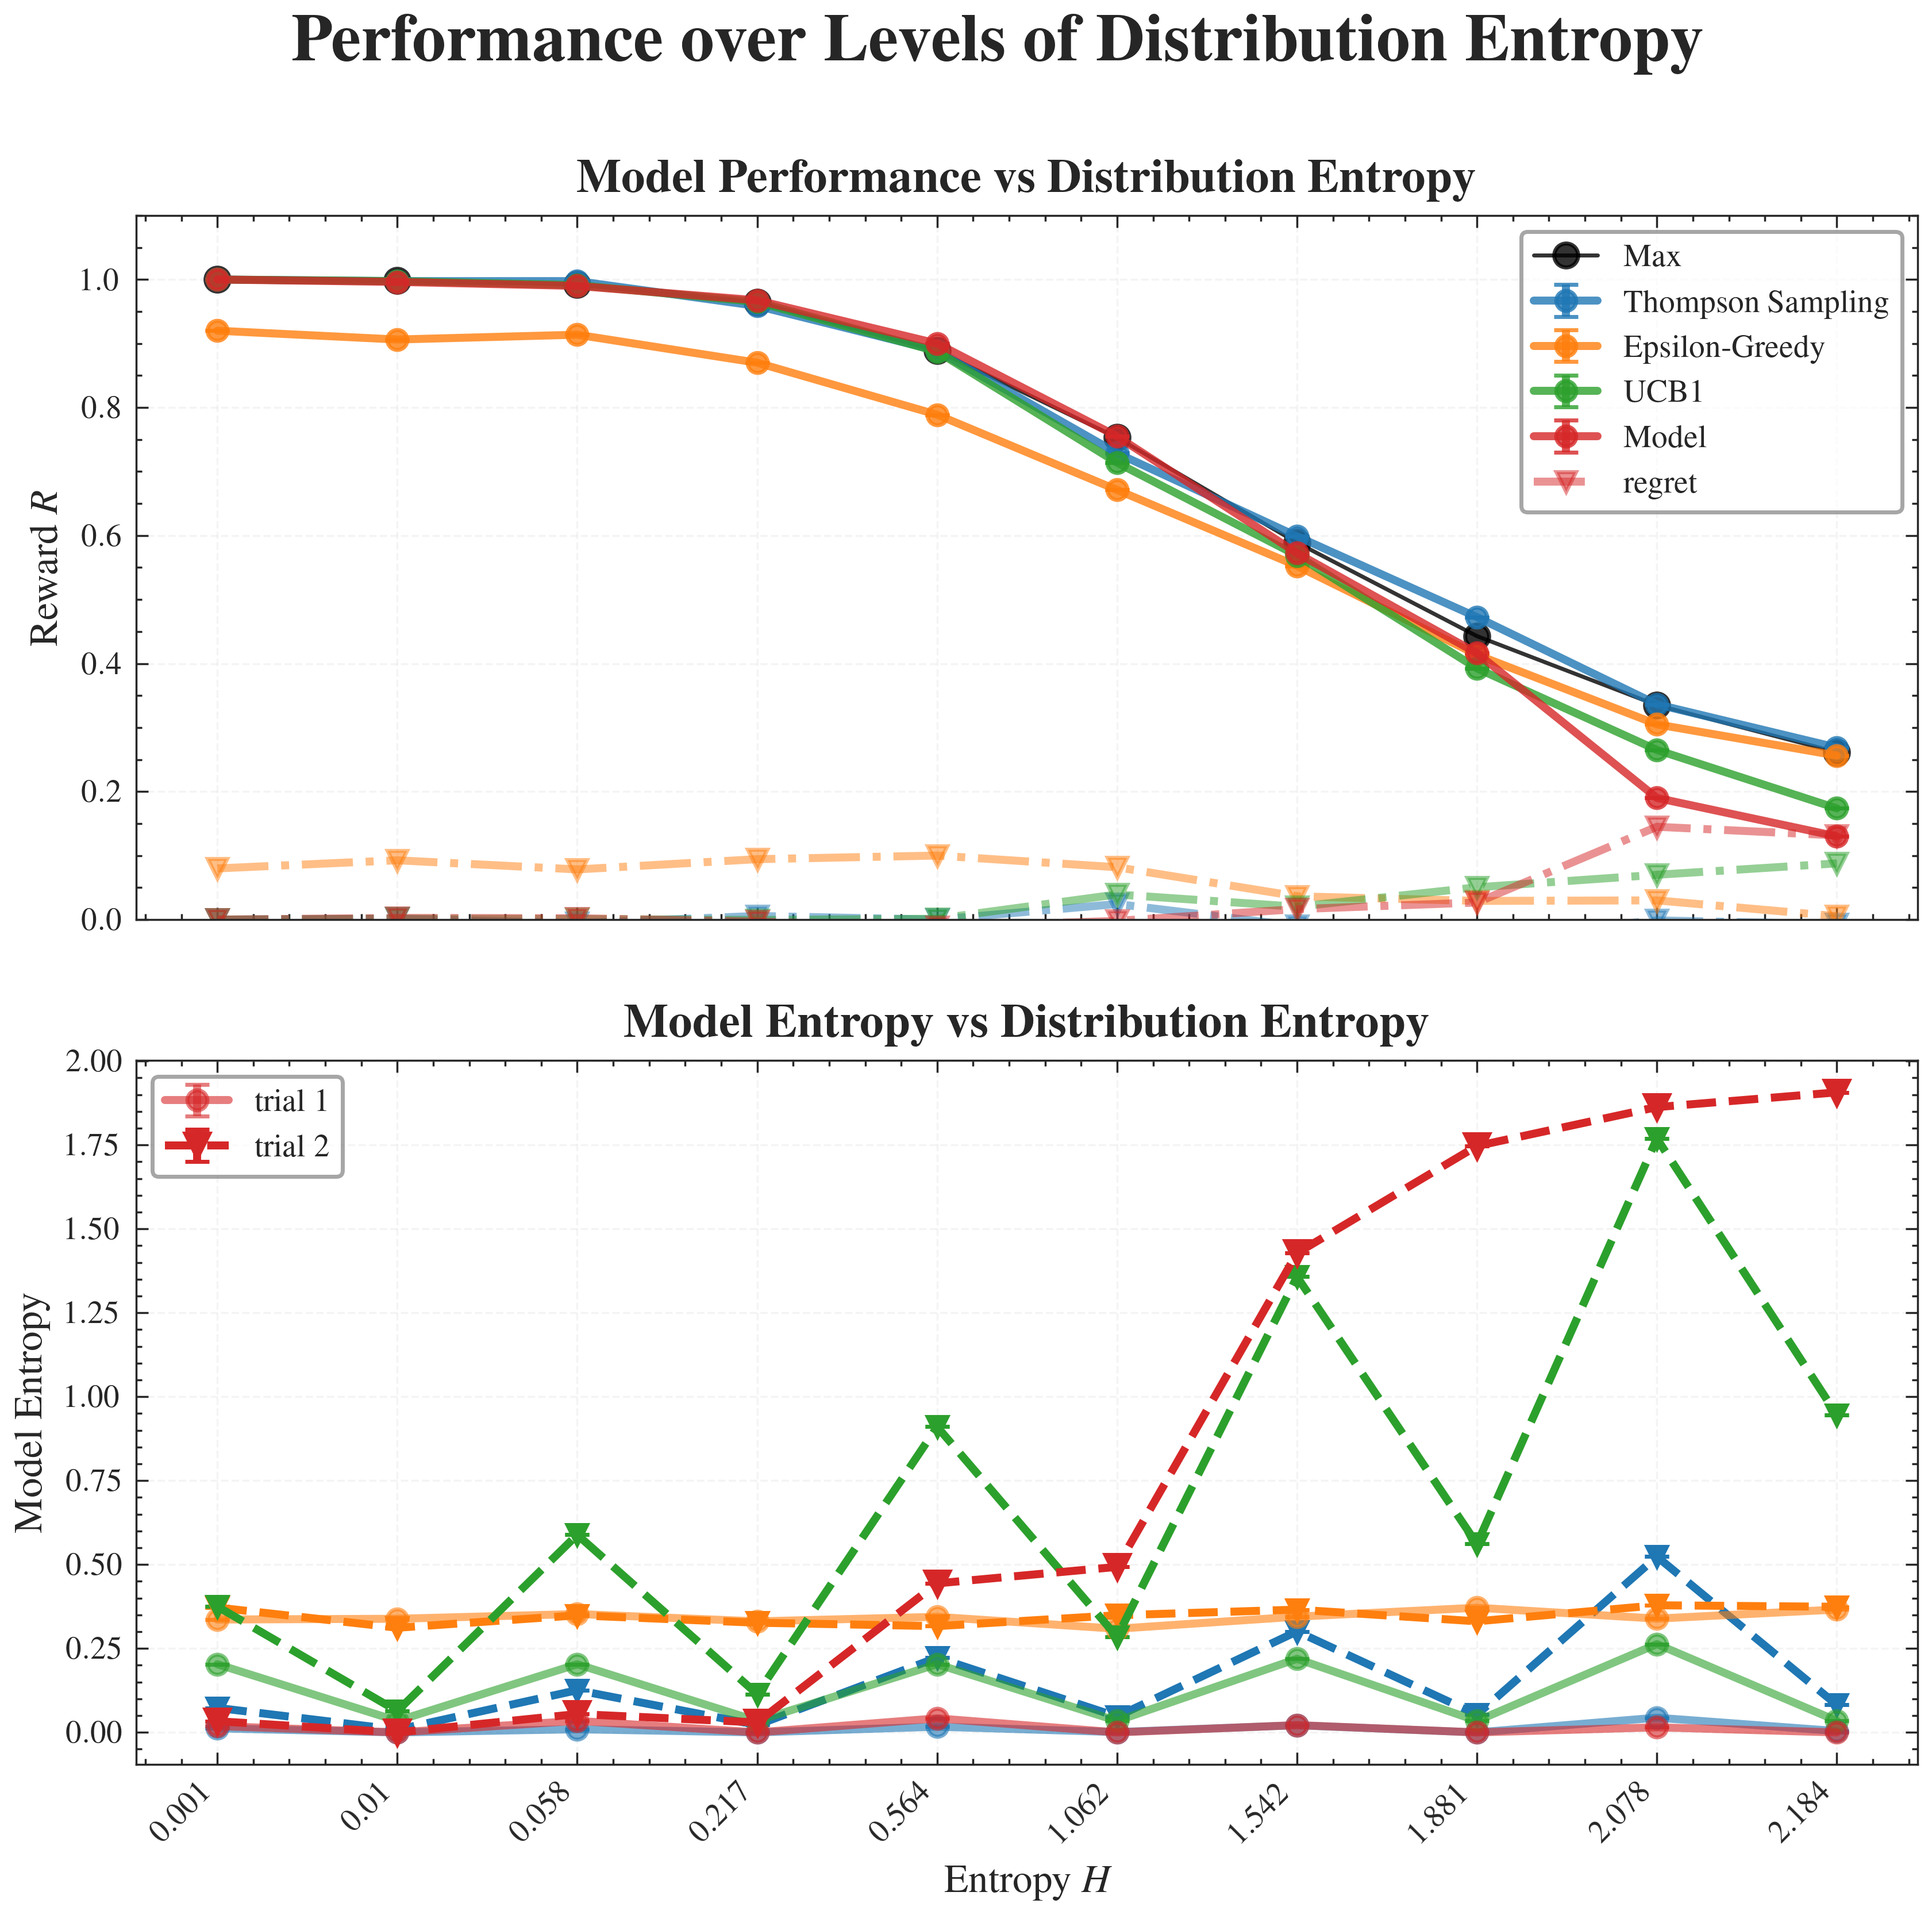
\includegraphics[width=0.9\textwidth]{figures/entropy_performance_plot.png}
    \caption{\textsc{Entropy analysis for the model in a stationary setting} - Top row: \textit{trial 1 and 2 have been divided into two columns. A solid line represents the average reward obtained by a model for increasing levels of entropy in the reward distribution; a dashed line instead reports the regret with respect to the upper bound (black solid line) }
- Bottom row: \textit{average entropy of the selections for the first and second trial of the simulation, each with 2000 rounds each (as calculated in \ref{sec:entropy}).}}
\end{figure}\label{fig:entropy_distr}




